\subsection{Hyperledger}

In Hyperledger Burrow the throughput was measured using the $Throughput_{alt}$ method mentioned in 2.1.
In \ref{table:4} the minimum, maximum and average time of a transaction is visualized. For 10 up to 1000 transactions
the minimum and average time of one transaction is below 1 second. The maximum time for more than 1000 transactions
drastically increases from 25 seconds to around 1000 seconds for 10000 transactions.

\begin{table}[!h]
\centering
\begin{tabular}{l|l|l|l|}
\hline
\multicolumn{1}{|l|}{\textbf{tx}} & \textbf{Min {[}s{]}} & \textbf{Max {[}s{]}} & \textbf{Avg {[}s{]}} \\ \hline
\multicolumn{1}{|l|}{\textit{10}} & \textit{0.436} & \textit{0.632} & \textit{0.530} \\ \hline
\multicolumn{1}{|l|}{\textit{100}} & \textit{0.379} & \textit{0.644} & \textit{0.475} \\ \hline
\multicolumn{1}{|l|}{\textit{1000}} & \textit{0.387} & \textit{25.557} & \textit{0.572} \\ \hline
\multicolumn{1}{|l|}{\textit{10000}} & \textit{0.359} & \textit{999.583} & \textit{3.457} \\ \hline 
\end{tabular}
\caption{Burrow: Min, Avg and Max execution time of a transaction}
\label{table:4}
\end{table}

The throughput for the test with 10 transactions as shown is figure \ref{fig:burrowtx10} shows a more or less
stable curve with only few up and downs and not much variation. The result for 100 (figure \ref{fig:burrowtx100})
transactions has a similar outcome. Starting the benchmark with 1000 (figure \ref{fig:burrowtx1000}) or even 10000
(figure \ref{fig:burrowtx10000}) transactions, the variance of some of these measurements is extremly high. In
the last test, the effect even intensifies with increased time passed.

\begin{minipage}{\linewidth}
    \makebox[\linewidth]{
    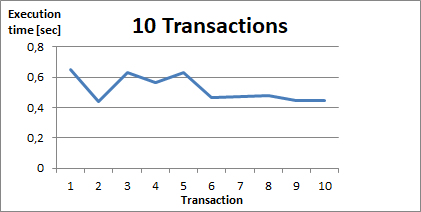
\includegraphics[width=0.75\textwidth]{img/10Tx.png}}
   \captionof{figure}{Burrow: 10 transactions and their execution time}\label{fig:burrowtx10}
\end{minipage}

\begin{figure}[!h]
    \centering
    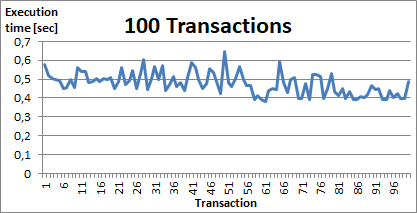
\includegraphics[width=0.75\textwidth]{img/100Tx.png}
   \caption{Burrow: 100 transactions and their execution time}
   \label{fig:burrowtx100}
\end{figure}

\begin{figure}[!h]
    \centering
    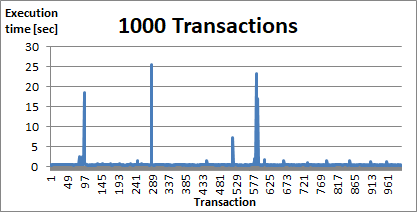
\includegraphics[width=0.75\textwidth]{img/1000Tx.png}
   \caption{Burrow: 1000 transactions and their execution time}
   \label{fig:burrowtx1000}
\end{figure}

\begin{figure}[!h]
    \centering
    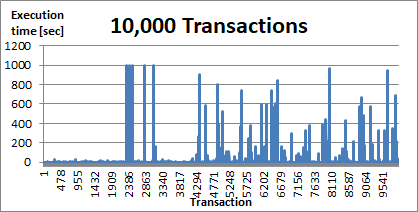
\includegraphics[width=0.75\textwidth]{img/10000Tx.png}
   \caption{Burrow: 10000 transactions and their execution time}
   \label{fig:burrowtx10000}
\end{figure}

\begin{figure}[!h]
    \centering
    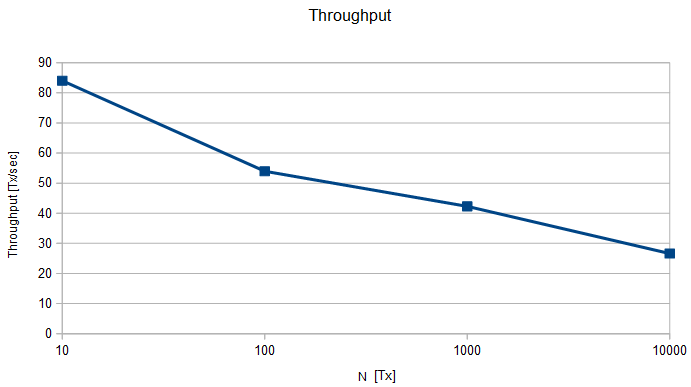
\includegraphics[width=0.75\textwidth]{img/Hyperledger.png}
   \caption{Burrow: Throughput}
   \label{fig:burrowthroughput}
\end{figure}